\thispagestyle{fancy}

\noindent
\begin{minipage}[t]{0.26\textwidth}
    \vspace{0pt}
    % Dóng hàng chính xác theo tọa độ: Hình 2 nằm cạnh phần cuối mục (c) và đoạn kiểm chứng đồ thị
    \vspace*{10.2cm}
    \centering
    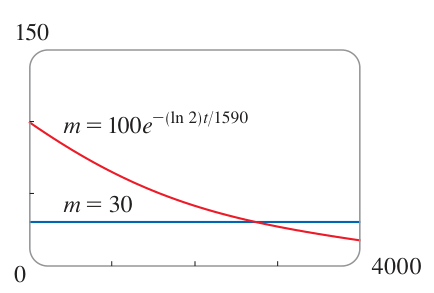
\includegraphics[width=\linewidth]{images/p0277_fig1.png}\\[4pt]
    {\small\textbf{\textsf{HÌNH 2}}}
\end{minipage}%
\hfill
\begin{minipage}[t]{0.71\textwidth}
    \vspace{0pt}
    Để xác định giá trị của $k$, ta sử dụng dữ kiện $m(1590) = \frac{1}{2}(100)$. Do đó
    \[
    100e^{1590k} = 50 \qquad \text{nên} \qquad e^{1590k} = \frac{1}{2}
    \]
    \noindent và \hfill $\displaystyle 1590k = \ln\frac{1}{2} = -\ln 2$ \hfill\mbox{}\\[8pt]
    \centerline{$\displaystyle k = -\frac{\ln 2}{1590}$}\\[8pt]
    \noindent Vì vậy \hfill $\displaystyle m(t) = 100e^{-(\ln 2)t/1590}$ \hfill\mbox{}\\[8pt]
    Ta có thể dùng tính chất $e^{\ln 2} = 2$ để viết biểu thức của $m(t)$ dưới dạng tương đương:
    \[
    m(t) = 100 \cdot 2^{-t/1590}
    \]
    \textbf{(b)} Khối lượng còn lại sau 1000 năm là
    \[
    m(1000) = 100e^{-(\ln 2)1000/1590} \approx 65\text{ mg}
    \]
    \textbf{(c)} Ta muốn tìm giá trị của $t$ sao cho $m(t) = 30$, tức là
    \[
    100e^{-(\ln 2)t/1590} = 30 \qquad \text{hoặc} \qquad e^{-(\ln 2)t/1590} = 0.3
    \]
    Ta giải phương trình này để tìm $t$ bằng cách lấy logarit tự nhiên ở cả hai vế:
    \[
    -\frac{\ln 2}{1590}\,t = \ln 0.3
    \]
    \noindent Do đó \hfill $\displaystyle t = -\frac{1590\ln 0.3}{\ln 2} \approx 2762\text{ năm}$ \hfill \textcolor{stewartcyan}{\rule{1.1ex}{1.1ex}}

    \vspace{0.8em}
    Để kiểm tra lại kết quả trong Ví dụ 2, ta sử dụng máy tính bỏ túi hoặc máy vi tính để vẽ đồ thị của $m(t)$ trong Hình 2 cùng với đường thẳng nằm ngang $m = 30$. Hai đường này cắt nhau khi $t \approx 2800$, và điều này phù hợp với kết quả ở phần (c).

    \vspace{1.2em}
    \noindent\raisebox{0.1ex}{\textcolor{stewartcyan}{\rule{1.1ex}{1.1ex}}}\hspace{0.5em}\textbf{Định luật làm nguội của Newton}\quad Định luật làm nguội của Newton phát biểu rằng tốc độ làm nguội của một vật thể tỉ lệ thuận với hiệu nhiệt độ giữa vật thể đó và môi trường xung quanh, với điều kiện hiệu số này không quá lớn. (Định luật này cũng áp dụng cho quá trình làm nóng.) Nếu ta gọi $T(t)$ là nhiệt độ của vật thể tại thời điểm $t$ và $T_s$ là nhiệt độ của môi trường xung quanh, thì ta có thể thiết lập Định luật làm nguội của Newton dưới dạng phương trình vi phân:
    \[
    \frac{dT}{dt} = k(T - T_s)
    \]
    trong đó $k$ là một hằng số. Phương trình này chưa hoàn toàn giống với Phương trình 1, vì vậy ta thực hiện phép đổi biến $y(t) = T(t) - T_s$. Do $T_s$ là hằng số, ta có $y'(t) = T'(t)$ và do đó phương trình trở thành
    \[
    \frac{dy}{dt} = ky
    \]
    Khi đó, ta có thể sử dụng Định lý 2 để tìm biểu thức cho $y$, từ đó xác định được $T$.

    \vspace{1.2em}
    \noindent\textcolor{stewartcyan}{\textbf{\textsf{VÍ DỤ 3}}}\hspace{1em}Một chai trà đá ở nhiệt độ phòng ($72^\circ\text{F}$) được đặt vào một tủ lạnh có nhiệt độ là $44^\circ\text{F}$. Sau nửa giờ, trà đã nguội xuống còn $61^\circ\text{F}$.
    \begin{enumerate}[label=\textbf{(\alph*)}, leftmargin=*, itemsep=2pt, topsep=4pt]
        \item Nhiệt độ của trà sau nửa giờ nữa là bao nhiêu?
        \item Mất bao lâu để trà nguội xuống còn $50^\circ\text{F}$?
    \end{enumerate}
\end{minipage}
